%# -*- coding: utf-8-unix -*-
%%==================================================
%% chapter01.tex for SJTU Master Thesis
%%==================================================

%\bibliographystyle{sjtu2}%[此处用于每章都生产参考文献]
\chapter{系统设计}
\label{chap:sys_design}

本章首先介绍基于SSD、HDD的混合存储系统qscache的设计动机与设计目标,然后展开描述了系统架构、数据映射策略、冷热数据识别策略、数据写回/迁移策略、最优化存储设备组合等设计。

\section{设计动机与设计目标}

\subsection{设计动机}

在上一章介绍了现在被广泛应用的三种开源混合存储系统flashcache、dm-cache和bcache,他们在性能、可靠性、内存开销等方面都有各自的优点与缺点,但有两个问题是这三个混合存储系统都未解决的。

第一个问题是这三个混合存储系统的最优化存储设备组合,他们都不支持将多存储设备与多后台设备统一为一个逻辑设备供用户使用。flashcache和dm-cache都仅支持单缓存设备对单后台设备,bcache支持单存储设备对多后台设备。对于普通用户而言,单个缓存设备已经足够应付正常的I/O负载,但对服务器级别的I/O负载来说,由于本身存储的数据量大,且I/O负载重,为了保证缓存的高命中率,缓存设备的容量也应相对数据量进行提升,但是如果混合存储系统仅支持单缓存设备,那么就需要单个大容量的缓存设备,成本会急剧上升,而如果混合存储系统支持多缓存设备,就可以以多个小容量的缓存设备实现大缓存容量,降低成本。

另一个问题是这三个混合存储系统都不支持针对不同进程设置不同权限,按权限分配进程的I/O带宽,由于系统整体的I/O带宽有限,在重负载情况下系统可能无法满足全部进程的I/O带宽要求,如果系统只是简单地将总I/O带宽平均分配给所有进程或者以先来先得的策略分配,可能会造成高权限的进程不如低权限进程的情况。为了解决这两个问题,需要设计一套新型混合存储系统,在保证系统的大容量、低成本、高性能的前提下实现对多缓存设备对多后台设备的支持以及对支持按进程权限分配I/O带宽的功能。

\subsection{设计目标}

本混合存储系统qscache的设计目标如下:

\begin{enumerate}
    \item 大容量。系统应具有较大的容量,且应能支持多缓存设备对多后台设备的缓存。
    \item 低成本。系统的存储成本应接近HDD的存储设备。
    \item 高顺序读写性能。系统的顺序读写性能应至少接近HDD的性能。
    \item 高随机读写性能。系统的随机读写性能应接近SSD的性能。
    \item 支持I/O带宽按权限分配。系统应支持按照进程的权限分配不同进程的I/O带宽。

\end{enumerate}

\section{系统架构}
\label{sec:qscache_architecture}

在\ref{chap:opensource_intro}中对不同的开源混合系统进行了对比分析,从系统性能和特性看,flashcache较dm-cache和bcache表现更为优秀,因此本文的qscache系统总体设计基于flashcache,系统总体架构如图\ref{fig:system_architecture}所示。系统首先将缓存设备与后台设备各自虚拟成一个统一的存储空间的虚拟缓存设备和虚拟后台设备进行管理,然后将虚拟缓存设备与虚拟后台设备虚拟为一个设备设备进行统一管理,并提供给用户使用。系统在接收到I/O请求后,通过映射机制将I/O进行分割,然后将分割后的I/O交给缓存管理模块,缓存管理模块首先进行存储地址查找,如果在缓存设备上则直接返回地址,否则进入数据冷热识别,并经缓存替换策略后发起缓存数据的更新操作。虚拟缓存设备和虚拟后台设备在收到请求后也经过存储位置查找,将对数据块的请求交给对应的真实设备处理。

\begin{figure}[H]
    \centering
    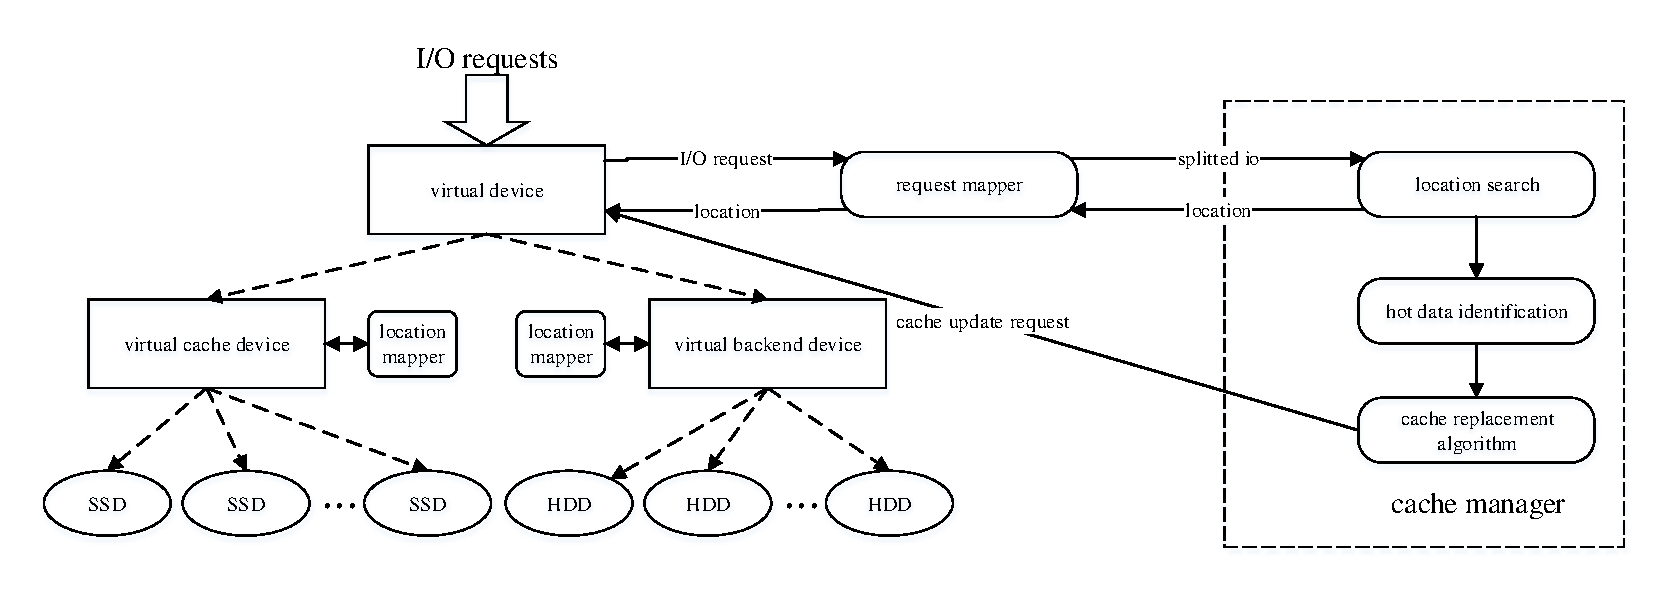
\includegraphics[width=\textwidth]{system_architecture.pdf}
    \bicaption[fig:system_architecture]{qscache系统整体架构}{qscache系统整体架构}{Fig.}{qscache overall system architecture}
\end{figure}

qscache系统整体采用分层架构,利用SSD较高的随机读写性能将SSD用作随机I/O缓存,将HDD作为源存储介质存储所有的数据,SSD上存储HDD中数据的子集,系统可用容量等于HDD的总容量。数据的流动规则如图\ref{fig:data_flow}所示,系统将随机I/O请求交由SSD处理,将随机I/O请求交由HDD处理,SSD与HDD之间进行数据的交换,HDD将热数据写入到SSD中提高系统整体的性能,SSD将被替换的数据写回到HDD中保证系统的一致性。

\begin{figure}[H]
    \centering
    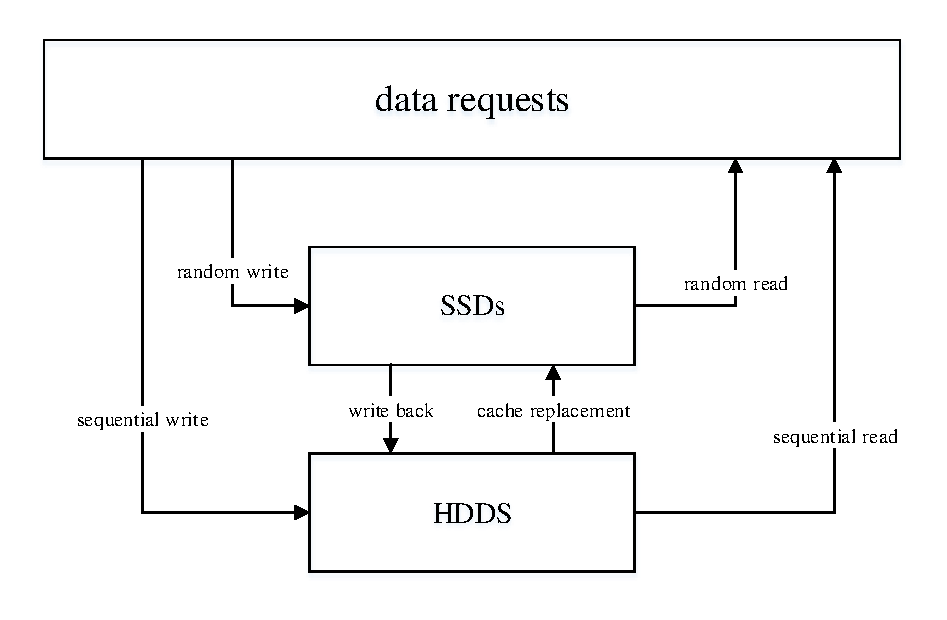
\includegraphics[width=0.8\textwidth]{data_flow.pdf}
    \bicaption[fig:data_flow]{数据流示意图}{数据流示意图}{Fig.}{data flow}
\end{figure}

\section{数据映射策略}
在\ref{sec:qscache_architecture}提到qscache系统采用的是缓存分层架构,将SSD分别作为HDD的随机I/O缓存。一般而言,在这种架构下,SSD上的数据是HDD上的子集,因此直接采用取模运算的映射方式比较方便,在\ref{sec:flashcache_mapping}介绍过flashCache正是使用了这种映射策略,下面将进一步介绍这种映射策略。 

\subsection{数据映射粒度}

与flashcache一样,qscache系统对数据的映射粒度也是块级(一般而言是4KB)。以块级映射数据的好处在于这种策略实现比较简单,并且对数据的处理粒度细,可以很好地找到真正的热数据,因此缓存的命中率会比较高。但是映射粒度细可能会导致将顺序请求拆散映射到不同设备的问题。并且系统的额外开销会更大,假设每个4KB的数据块需要20bytes的元数据进行管理,那么一块100GB的SSD被用作缓存设备,约需要500MB的额外开销用来管理元数据,并且为了保证对元数据处理的高效性,肯定是将元数据放在内存中,一般缓存设备容量与后台设备容量比约为1:10,那么100GB的SSD用作缓存设备,后台设备大约就是一块1TB的HDD,相当于整个系统是构建在普通台式机中,而一般台式机的内存约4GB-16GB,那么这部分额外开销约占3.125\%到12.5\%,如果这台机器只是作为存储设备,那么这个开销相对来说还可以接受。当然,后台设备的容量越大,相应地为了保证缓存的高命中率,缓存设备的容量也要扩大,相应的额外开销也会变大,当后台设备容量达到PB级,缓存设备的容量将达到TB级,而额外的内存开销将达到GB级,这就不是那么可接受了。但是综合考虑块级映射的利弊以及实现难度,本文最后还是采用块级映射的策略,对于额外内存开销的问题留待以后的研究解决。

\subsection{数据映射规则}

qscache系统的映射规则同样采用组映射的方式,具体映射公式为公式\ref{eq:dbn_to_set},其中dbn为数据块的起始扇区,target set为被映射到的set,block size为数据块大小,set size是每个set包含的数据块数,set number指缓存设备可以包含多少个set。以100GB的缓存设备容量为例,取数据块大小为4KB,每个set包含512个数据块,那么缓存设备总共可以有50000个set。

采用组相联映射的好处在于一定大小的连续的数据块会被映射到相同的set,这样在缓存设备中这些数据块也是连续存放的,这样对于顺序请求就不容易出现被打散到不同设备上进行处理的情况,

\section{冷热数据识别策略}
\label{sec:data_hot_identification}

qscache系统的冷热数据识别采用双层LRU链表的方法。通过使用两个LRU链表分别表示hot和warm,当数据没有命中时首先将其放到warm链表中,当对该数据的访问达到一定阈值时才将其放到hot链表中,缓存块的替换发生在warm链表,当需要替换warm链表中的数据时,对应的缓存块发生替换,同时将hot链表的尾放入warm链表中。使用双层LRU链表的好处,一个在于实现比较简单,对于链表的操作只需要操作指针即可,另一个在于使用双层LRU链表当发生大量的遍历型I/O请求时并不会导致大量的缓存失效。

\section{数据写回/迁移策略}

在系统运行的过程中,会遇到数据块在缓存设备和后台设备中版本不一致的情况,这时候就需要对数据块进行写回/迁移。在qscache系统中缓存块的元数据中使用cache\_state表示该缓存块的状态,状态标志位共有:VAILD(表示缓存设备与后台设备的数据一致),INVALID(表示后台设备中的数据为最新),DIRTY(表示缓存设备中的数据为最新),DISKREADINPROG(表示正在从后台设备读取数据),DISKWRITEINPROG(表示正在向后台设备写入数据),CACHEREADINPROG(表示正在从缓存设备读取数据),CACHEWRITEINPROG(表示正在向缓存设备写入数据),DIRTY\_FALLOW\_1(表示准备被清理的候补的候补),DIRTY\_FALLOW\_2(表示准备被清理的候补),缓存块的状态可能同时包含上述多个标志位。

qscache系统对数据块是否需要写回,除了依据冷热数据识别策略对需要替换出去的缓存块进行写回操作外,还会对长期被缓存在缓存中的数据块进行写回操作,对这些数据的识别是周期性执行的,每过一个周期,系统会对有DIRTY标志且没有DISKREADINPROG、DISKWRITEINPROG、CACHEREADINPROG、CACHEWRITEINPROG标志(即该数据块目前并没有被操作)的数据块判断是否有DIRTY\_FALLOW\_1标志,如果没有则给它加上DIRTY\_FALLOW\_1标志,如果有则加上DIRTY\_FALLOW\_2标志,同时有DIRTY\_FALLOW\_1标志与DIRTY\_FALLOW\_2标志的数据块就是准备被清理的候补。在该数据块被写回前如果被使用,则去除DIRTY\_FALLOW\_1标志与DIRTY\_FALLOW\_2标志。

qscache系统触发写回操作,除了在缓存块需要被替换时触发外,对于长期处于缓存中而没被使用的数据块,在经过定期检测加上标志后,会在每次I/O操作时通过I/O操作的回调函数对这些数据块进行清理操作。


\section{最优化存储设备组合}

\label{sec:multi-cache_to_multi-backend}

在系统架构中可以看到,qscache系统对于多缓存设备和多后台设备的管理采用增加一层虚拟层的策略。系统不直接将多个缓存设备和多个后台设备统一为一个虚拟设备进行管理以供用户使用,而是首先将多个缓存设备统一成一个虚拟缓存设备,将多个后台设备统一成一个虚拟后台设备。

分层管理通过增加中间层,相比直接管理多个设备,系统可以将设备管理策略与系统架构、数据映射策略、冷热数据识别策略、数据写回/迁移策略等缓存策略隔离开,使策略的配置更简单。例如,如果要保证多个缓存设备的容量被均衡地使用,在直接管理下,相应的数据映射策略和数据写回/迁移策略都要对应修改,但在分层管理下,数据映射策略和数据写回/迁移策略可以维持不变,只需要改变设备管理策略,将多个设备以raid0生成对应虚拟设备即可。如果要保证数据的可靠性,配置多副本,则在直接管理下,需要将设备分组管理、分组操作,对应的各种操作都需要改变,而在分层管理下只需要以raid1配置设备即可。

分层管理虽然在策略配置上更灵活,但相比直接管理,系统在扩容上会略显不足。在直接管理下,对系统的扩容可以实现热扩容,即在系统运行的状态直接进行扩容操作,直接增加被管理的设备并更新对应的参数变化即可。与之相对,在分层管理下,由于设备管理与其它部分隔离,为了保证扩容后系统的正确性,需要先将虚拟缓存设备的数据全部写回虚拟后台设备,然后禁用缓存,对系统进行扩容,再开启缓存,系统整体会有性能下降的一段时间,且影响时间与被缓存的数据量有关,即约与虚拟缓存设备的容量成正比。

本文的研究认为,对于普通用户而言,系统基本不存在扩容这一行为,而对于服务器级用户而言,扩容也并不是一种经常进行的行为,但是对于设备管理策略的变更的频率确是相对而言比较高的。设备管理的策略主要与系统的I/O负载类型有关,变化比较多样,有的可能只是要求设备负载均衡,有的可能只是要求能提供灾备,但有的可能会很复杂,是多种简单策略的组合。如果采用直接管理的模式,虽然也能实现各种策略,但是对应的代码修改量会十分巨大,分层管理则可利用现有的技术如逻辑盘卷管理(LVM, Logical Volume Manager)\cite{wada2009logical}完成。

\section{I/O带宽按权限分配}

qscache系统通过对不同进程按照各自权限分配IOPS来限制不同进程的I/O带宽,采用CFQ(Completely Fair Queuing)策略,如图\ref{fig:system_io_scheduler}所示,每个进程都被分配一个队列,每个I/O请求被放到对应进程的队列中,根据每个进程的权限不同,给每个进程的I/O请求分配不同的时间片数量,每个时间片取出I/O请求通过映射到实际设备进行请求处理。

\begin{figure}[!htbp]
    \centering
    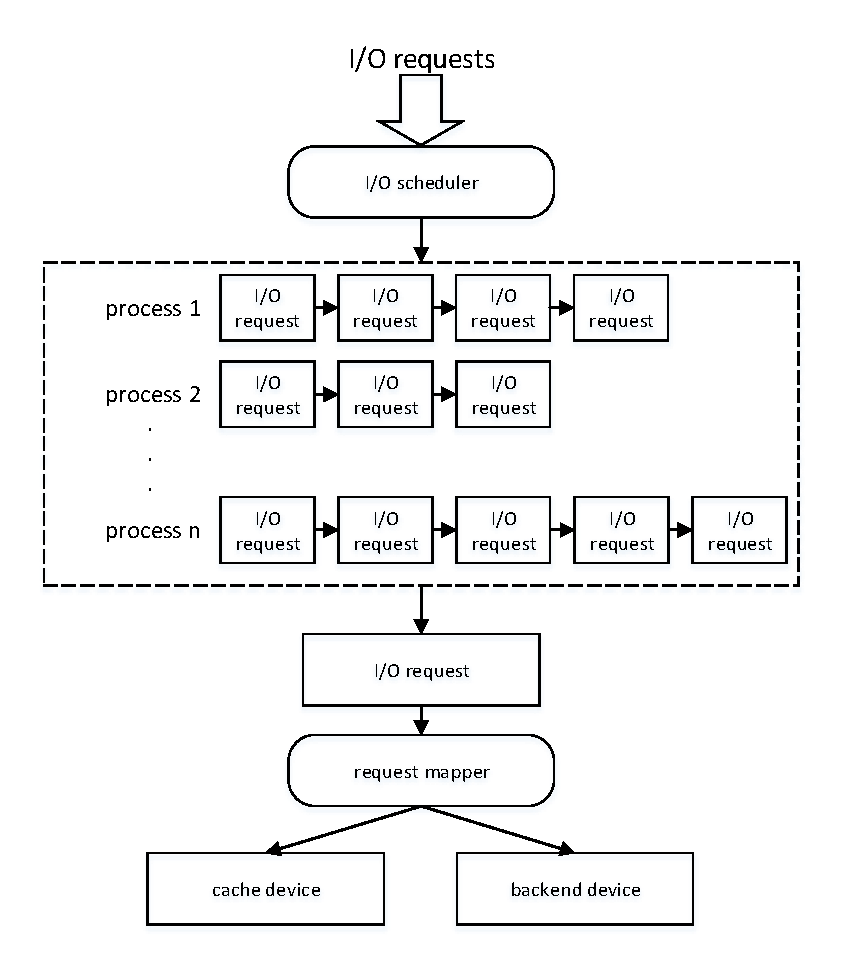
\includegraphics[width=0.8\textwidth]{system_io_scheduler.pdf}
    \bicaption[fig:system_io_scheduler]{I/O带宽分配流程}{I/O带宽分配流程}{Fig.}{I/O bandwidth quota process}
\end{figure}

\section{本章小结}

本章介绍了qscache系统在设计过程中所遇到的问题以及对分析与解决思路。介绍了qscache系统的设计动机与设计目的,并对优化存储设备组合与I/O带宽按权限分配等问题的策略选择进行了分析,为接下来的qscache系统实现做准备。